%
% Chapter 8
%

\chapter{Statistical Methods and Systematic Uncertainties}
\label{sig_ext}
% \epigraph{Statistics is the grammar of science.}{\textit{Karl Pearson}}
% \vskip 0.5in

\section{Introduction}
In the search for LFV Higgs decays, a discovery will be the observation of events with the Higgs Boson decaying either into \mutau or \etau. As the LFV is forbidden in SM, the SM can be taken as the background model, and discovery can be claimed if the observation is not compatible with this background model. The uncertainties resulting from theoretical, experimental, and statistical sources can give rise to an excess in the observation even when there is no signal at all. When an excess is observed, a p-value is computed. The p-value represents the probability that an observed excess is due to statistical fluctuations. The p-value has to be very low to indicate that the excess observed is due to a signal's presence and not merely a statistical fluctuation. However, if no excess is observed, upper exclusion limits can be set on the branching fraction. This chapter describes the statistical methods used for extracting the signal strength, followed by the systematic uncertainties involved in the analysis.

\section{Statistical methods}
\label{stat_meth}

The results on the branching fraction of the LFV Higgs-boson decays to \mutau, and \etau are estimated using a profile likelihood method. The SM Higgs boson production cross-sections are used for the signal model, while the branching fraction of the Higgs boson to \mutau and \etau remain free parameters. The branching fraction is the parameter of interest. In addition to it, the signal and background model contain in general nuisance parameters whose values must be derived from collision data. The profile likelihood method is implemented, assuming the asymptotic approximation. Distributions of the BDT discriminator and the collinear mass for signal and various background processes are fitted to collision data. Systematic uncertainties are represented as nuisance parameters, and they can affect the normalization or the shape of the distribution.

Poisson distribution can be used to model the expected number of events and the observed events for the situation at hand. The expected number of events is $\mu\cdot s + b$, where $s$ is the expected signal event yields, and $b$ is the expected background event yields. The parameter $\mu$ is the signal strength modifier, which changes the signal production cross-sections of all the production mechanisms by exactly the same scale of $\mu$. The likelihood function measures the goodness of fit of a statistical model to a sample of data for given values of the unknown parameters. For our situation, the likelihood function $\mathcal{L}(data|\mu)$ is then given by:
\begin{equation}
  \mathcal{L}(data|\mu)=\prod_{i=1}^{bins}\frac{(\mu\cdot s_i + b_i)^{n_i}}{n_{i}!}e^{-\mu\cdot s_i - b_i}
\end{equation}
where $n_i$ is the number of events observed in the bin i of the distribution, and $s_i$ and $b_i$ are expected number of signal and background events in that bin, respectively.

The nuisance parameters which represent the systematic uncertainties are embedded into the likelihood function. The uncertainties considered are taken to be 100\%-correlated or uncorrelated, thus ensuring that the likelihood function has a clean factorized form ~\cite{ATLAS:2011tau}. However, certain uncertainties have partial correlations across the years. There are also partial correlations among uncertainties between the embedded and MC samples. A partially correlated uncertainty is separated into 100\%-correlated or uncorrelated components.
The magnitude of the correlated component will be $\rho$, and for the uncorrelated part, it will be $\sqrt{1-\rho^{2}}$, where $\rho$ is the magnitude of the correlation. For example, a 50\% correlation will have a correlated component with 0.5 as magnitude and an uncorrelated part with 0.866 as magnitude.

The expected signal and background yields are effected by nuisance parameters and we parametrize them as $s(\theta)$ and $b(\theta)$. There is a default value $\tilde{\theta}$ for each component of $\theta$. The default value reflects our degree of belief on the real value of $\theta$. The probability distribution function (pdf) $\rho(\theta|\tilde{\theta})$ can then be interpreted as a posterior distribution from measurements of $\tilde{\theta}$. Using Bayes' theorem:
\begin{equation}
  \rho(\theta|\tilde{\theta})=\rho(\tilde{\theta}|\theta)\cdot\pi_\theta(\theta),
\end{equation}
The priors $\pi_\theta(\theta)$ are taken as flat distributions representing no prior knowledge of $\theta$. The likelihood of the measurement can be constrained by using the pdf of $\tilde{\theta}$. After incorporating the nuisance parameters, the likelihood function now becomes:
\begin{equation}
  \mathcal{L}(data|\mu,\theta)=\prod_{i=1}^{bins}\frac{(\mu\cdot s_i(\theta) + b_i(\theta))^{n_i}}{n_{i}!}e^{-\mu\cdot s_i(\theta) - b_i(\theta)}\cdot\rho(\tilde{\theta}|\theta)
\end{equation}

If no excess is observed then upper exclusion limits can be set on the branching fraction using the CL$_\text{s}$ method ~\cite{Read:2002hq, Read:2000ru, Junk:1999kv}. According to Neyman-Pearson lemma, the likelihood ratio is the most powerful discriminator. The likelihood ratio is used generally in the searches at the LHC for hypothesis testing, and it uses profiling of nuisances. The test statistic is denoted by $\tilde{q_\mu}$ and is given by:
\begin{equation}
\label{eq:proflik}
  \tilde{q_\mu}=-2\text{ ln}\frac{\mathcal{L}(\text{data}|\mu,\hat{\theta_\mu})}{\mathcal{L}(\text{data}|\hat{\mu},\hat{\theta})},\text{   with  } 0 \leq \hat{\mu} \leq \mu
\end{equation}
where $\hat{\theta_\mu}$ refers to the conditional maximum likelihood estimators of $\theta$, while $\hat\mu$ and $\hat\theta$ refer to the global maximum likelihood estimators for $\mu$ and $\theta$. The constraint $0 \leq \hat{\mu}$ ensures that the signal rate cannot be negative. In contrast, the upper constraint $\hat{\mu} \leq \mu$ is imposed to guarantee that upward fluctuations of data such that $\hat{\mu} > \mu$ are not considered as evidence against the signal hypothesis.

The observed value of the test statistic, $\tilde{q_\mu}^{obs}$, is calculated for the signal strength $\mu$, using equation~\ref{eq:proflik}. Maximum likelihood estimators for the nuisance parameters, under the background-only and signal-plus-background hypotheses, are calculated and are denoted by $\hat{\theta_{0}}^{obs}$ and $\hat{\theta_\mu}^{obs}$ respectively. They are used to generate toy Monte Carlo pseudo-datasets. These pseudo datasets are used to construct pdfs of test statistics $f(\tilde{q_\mu}|0,\hat{\theta_{0}}^{obs})$ and $f(\tilde{q_\mu}|\mu,\hat{\theta_\mu}^{obs})$ by treating them as if they were real data. An illustration of these distributions can be seen in Figure ~\ref{fig:test_stat_dist}.
\begin{figure*}[!htpb]\centering
 \captionsetup{width=.87\textwidth,justification=centering}
 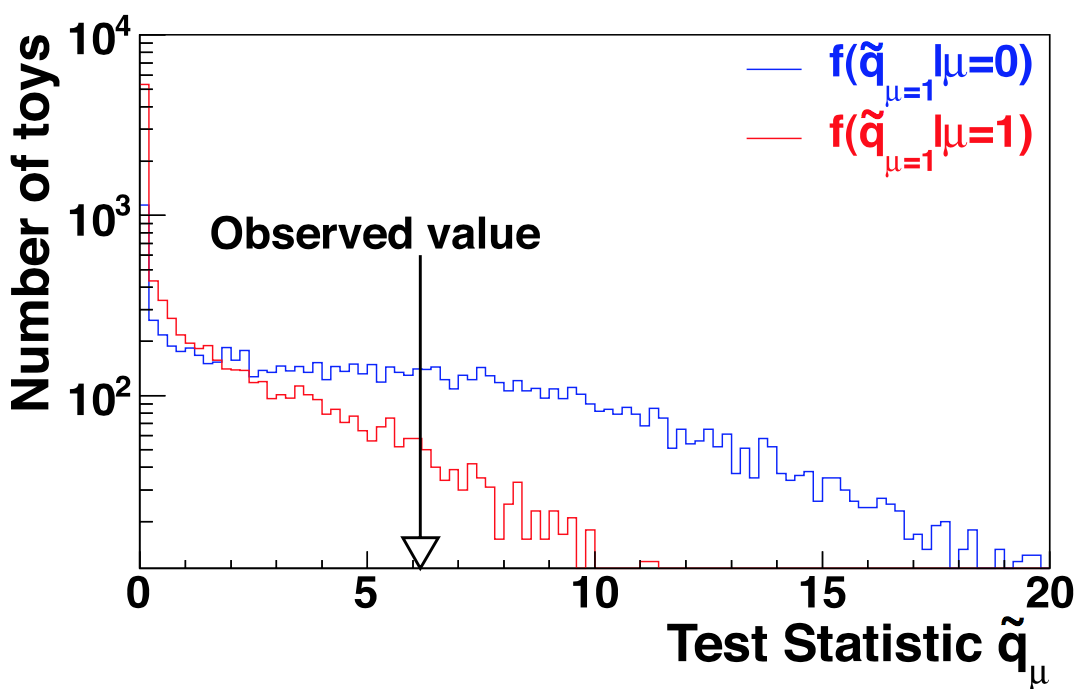
\includegraphics[width=0.85\textwidth]{plots/chapter8/test_statistic_distri.png}
 \caption{Test statistic distributions for ensembles of pseudo-data generated for background-only (blue) and signal-plus-background (red) hypotheses~\cite{ATLAS:2011tau}.}
 \label{fig:test_stat_dist}
\end{figure*}

CL$_\text{s+b}$ and CL$_\text{b}$ correspond to the probabilities of the observations under both hypotheses. CL$_\text{s+b}$ measures the incompatibility of data under the signal-plus-background hypothesis. CL$_\text{b}$ measures the incompatibility of data under the background hypothesis. These quantities alone are not adequate for hypothesis testing. For example, in situations when the signal is so small that both hypotheses are compatible with the observation and a downward fluctuation of the background can lead to an inference of signal. Also, the incompatibility of the data with the background-only hypothesis alone doesn't tell us that it is indeed compatible with the signal. The ratio of the two quantities referred to as CL$_\text{s}$ helps deal with both the situations described above well. The 95\% CL is then arrived at by iterating over $\mu$ until we have CL$_\text{s}=0.05$. The $\mu$ thus obtained is denoted as $\mu^{95\%CL}$ and is said to be excluded at 95\% CL.

\begin{gather}
  p_\mu=P(\tilde{q_\mu}\geq \tilde{q_\mu}^{obs}|\text{signal-plus-background})=\int_{\tilde{q_\mu}^{obs}}^{\inf}f(\tilde{q_\mu}|\mu,\hat{\theta_\mu}^{obs})d\tilde{q_\mu} \\
  1-p_b=P(\tilde{q_\mu}\geq \tilde{q_\mu}^{obs}|\text{background-only})=\int_{\tilde{q_\mu}^{obs}}^{\inf}f(\tilde{q_\mu}|0,\hat{\theta_0}^{obs})d\tilde{q_\mu} \\
  \text{CL}_\text{s}=\frac{p_\mu}{1-p_b}
\end{gather}

The discussion until now pertains to calculating the observed limits when the data is unblinded. However, when the analysis is performed in a blinded manner, we first calculate the expected limits, which are upper exclusion limits calculated using toy datasets of background-only expectation. An extensive set of pseudo-data is generated using the background-only hypothesis, and CL$_\text{s}$ and $\mu^{95\%CL}$ is calculated for each of them. A distribution is built as a function of the $\mu^{95\%CL}$ calculated for each of these pseudo-data. We then calculate the median expected limit from the 50\% quantile of the cumulative distribution function. The $\pm 1\sigma$ and $\pm 2\sigma$ bands are calculated similarly by integrating the distribution until the appropriate quantiles are reached. The expected limits can be used to maximize the sensitivity of the search. A more stringent median limit corresponds to a more sensitive search.

\begin{figure*}[!htpb]\centering
  \captionsetup{width=.87\textwidth,justification=centering}
  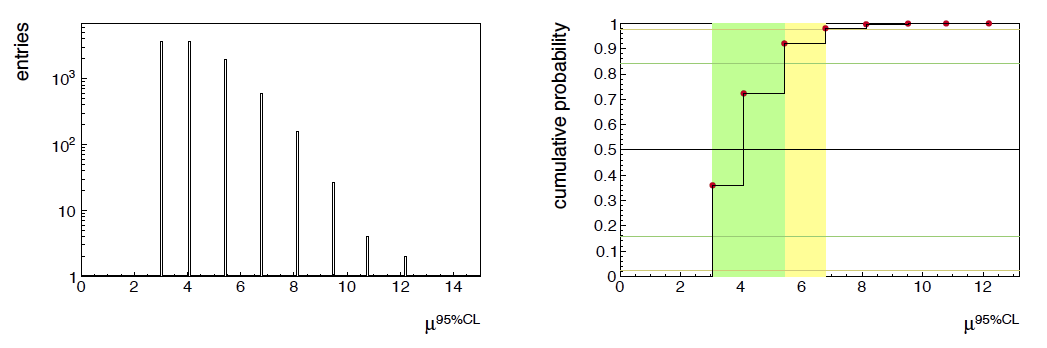
\includegraphics[width=0.85\textwidth]{plots/chapter8/Median.png}
  \caption{(Left) An example of differential distribution of possible limits on $\mu$ for the background-only hypothesis. (Right) The cumulative probability distribution of the plot on the left with 2.5\%, 16\%, 50\%, 84\%, and 97.5\% quantiles defines the median expected limit as well as the 68\% and 95\% bands for the expected value of $\mu$ for the background-only hypothesis.}
  \label{fig:median}
\end{figure*}

\section{Systematic Uncertainties}

Several sources of experimental and theoretical systematic uncertainties are taken into account as input to the maximum likelihood fit. These uncertainties affect both the normalization and the shape of the distributions of the different processes. The normalization effect is described by log-normal pdfs and corresponds to a multiplicative factor in the signal or background yields. These pdfs are characterized by the parameter $\kappa$ and are well-suited for positively valued observables. The log-normal distribution looks like:
\begin{equation}
\rho(\theta|\tilde{\theta})=\frac{1}{\sqrt{2\pi}\text{ ln}(\kappa)}\text{exp }(\frac{\text{ln}(\theta/\tilde{\theta})^2}{2(\text{ln }\kappa)^2}) \frac{1}{\theta}
\end{equation}

The distributions' shape is altered when the systematic uncertainties affect the scale of the distribution differently in each bin. Such uncertainties are called shape uncertainties ~\cite{Conway:2011in} and are modeled using a linear interpolation method ~\cite{Read:1999kh}. Two other distributions obtained by varying the nuisance parameter by $\pm 1$ standard deviation are used for implementing the shape uncertainties. A parameter is added to the likelihood that smoothly interpolates between these two other distributions.

As the analysis is categorized into different final states, partial and complete correlations between the uncertainties in different categories are treated appropriately and are summarized in Tables ~\ref{tab:systematics_mt} and ~\ref{tab:systematics_et}.

\begin{table}[htpb]
\centering
\caption{Systematic uncertainties in the expected event yields for the \Hmt channels.}
\begin{tabular}{lcc}
\hline
Systematic Uncertainty             &        \muhad           &       \mue       \\
\hline
Muon Identification/Isolation      &          2\%            &       2\%        \\
Electron Identification/Isolation  &         \NA             &       2\%        \\
Trigger                            &          2\%            &       2\%        \\
\tauh Identification               &  \pt\, dep. (2--3\%)    &       \NA        \\
$\Pgm \to \tauh$ Identification    &       10--70\%          &       \NA        \\
b-tagging veto                     &       $<$ 6.5\%         &     $<$ 6.5\%    \\
Prefiring                          &     (0.2--1.3\%)        &   (0.2--1.3\%)   \\
Jet energy scale                   &       3--20\%           &     3--20\%      \\
and resolution                     &                         &                  \\
\tauh energy scale                 &      0.7--1.2\%         &       \NA        \\
$\Pe \to \tauh$ energy scale       &        1--7\%           &       \NA        \\
$\Pgm \to \tauh$ energy scale      &         1\%             &       \NA        \\
\Pe\ energy scale                  &         \NA             &     1--2.5\%     \\
\Pgm\ energy scale                 &      0.4--2.7\%         &    0.4--2.7\%    \\
Unclustered energy scale           &    $\pm 1 \sigma$       &  $\pm 1 \sigma$  \\
\hline
\end{tabular}
\label{tab:systematics_mt}
\end{table}

\begin{table}[htpb]
\centering
\caption{Systematic uncertainties in the expected event yields for the \Het channels.}
\begin{tabular}{l*{4}{c}}
\hline
Systematic Uncertainty             &        \ehad            &       \emu       \\
\hline
Muon ID/Isolation                  &         \NA             &       2\%        \\
Electron ID/Isolation              &         2\%             &       2\%        \\
Trigger                            & 2\% for SingleElectron, &       2\%        \\
                                   &  5\% for Cross-Trigger  &                  \\
\tauh Identification               &   \pt dep. (2-–15\%)    &       \NA        \\
$\Pe \to \tauh$ ID                 &         40\%            &       \NA        \\
b-tagging veto                     &       $<$ 6.5\%         &     $<$ 6.5\%    \\
Prefiring                          &     (0.2--1.3\%)        &   (0.2--1.3\%)   \\
Jet energy scale                   &       3--20\%           &     3--20\%      \\
and resolution                     &                         &                  \\
\tauh energy scale                 &      0.7--1.2\%         &       \NA        \\
$\Pe \to \tauh$ energy scale       &        1--7\%           &       \NA        \\
$\Pgm \to \tauh$ energy scale      &         1\%             &       \NA        \\
\Pe\ energy scale                  &       1--2.5\%          &     1--2.5\%     \\
\Pgm\ energy scale                 &         \NA             &    0.4--2.7\%    \\
Unclustered energy scale           &    $\pm 1 \sigma$       &  $\pm 1 \sigma$  \\
\hline
\end{tabular}
\label{tab:systematics}
\end{table}


The uncertainties to reconstruct a \tauh and estimation of its identification efficiency for different \pt\, ranges are measured using a tag-and-probe method and found to be in the range of 2-3\%. The uncertainties for different ranges of \pt\, are treated in an uncorrelated way. These uncertainties are also considered for the embedded \Pgt{}\Pgt\, background, where they are treated 50\% correlated with the simulation uncertainties. For the embedded samples, triggering on muons before being replaced by \Pgt\, leptons have an uncertainty of about 4\%. This uncertainty is treated as uncorrelated between the three years due to different triggering criteria. Uncertainty due to tracking measurement is also considered in correlated way between $h^{\pm}$ and $h^{\pm}h^{\mp}h^{\pm}$ decay modes and uncorrelated way between $h^{\pm}\pi^{0}$ and $h^{\pm}h^{\mp}h^{\pm}\pi^{0}$ decay modes.

Uncertainties due to electrons and muons misidentified as \tauh candidates correspond to 40\% and between 10-70\%, respectively, for different bins of \pt, $\eta$, and \tauh decay modes. The uncertainty due to \tauh energy scale uncertainty is treated as uncorrelated for different decay modes and 50\% correlated between embedded and simulated backgrounds and ranges from 0.7 to 1.2\%. The uncertainty due to the electron (muon) energy scale for misidentified leptons is independent of the \tauh energy scale and amount to 7\% (1\%). The effect of lepton energy resolution is found to be negligible for the study under consideration.

The jet energy scale (JES) is affected by several sources, and uncertainty due to them is evaluated as a function of \pt\, and pseudorapidity. JES's effect is propagated to the BDT discriminator by varying each source of uncertainty by one standard deviation and disseminating them to the fit template for each process and are of the order of 3-20\%. The jet energy resolution uncertainties are also taken into account, and they mostly impact the \mjj-defined categories. In the particle flow candidate list, jets with $\pt < 10\GeV$ are not considered. They fall under unclustered energy. The unclustered energy scale is considered independently for charged particles, neutral hadrons, photons, and very forward particles, affecting both shape and yield, and are treated as uncorrelated. The efficiency to classify a jet as b-tagged is different in data, and simulation and scale factors depend on jet \pt\, and $ \eta $ are used to correct simulation. The uncertainties in measuring these scale factors are treated as a systematic uncertainty.

The uncertainty to track leptons (\Pe, \Pgm), reconstruct them, and identify and isolate is measured using the tag-and-probe method in data in \Zee and \Zmm events and sums up to about 2\% ~\cite{Chatrchyan:2012xi, Khachatryan:2015hwa, Khachatryan:2015dfa, CMS:2016gvn}. The uncertainty in the measurement of the muon momentum scale is in the range $0.4-2.7\%$ for different $\eta_\Pgm$, while for the electron momentum scale, it is less than 1\%. The selection of events using electron and muon based triggers results in additional 2\% uncertainty in the yield of simulated processes.

The misidentification rates in the \ehad and \muhad final states are parameterized using a linear function on \tauh \pt. There are a couple of uncertainties that are ascribed per fit function. The normalization uncertainties in the data-driven estimations of misidentified-lepton backgrounds ($\text{jet}\to\tauh, \Pgm, \Pe$), is taken from the orthogonal control region as described in Chapter ~\ref{bg_val}. Discriminators with different signal to background efficiency are used to single out  \tauh against electrons and muons, which entails an additional 3\% uncertainty for the \ehad channel. The misidentified lepton background in the \emu and \mue final states is affected by different shape uncertainties. The statistical uncertainties arising from both fits of the OS/SS extrapolation factor as a function of the spatial separation between \Pe\, and \Pgm\, and lepton \pt\, are taken into account. The uncertainties from OS/SS extrapolation factor are estimated in the anti-isolated muon control region, which results in an additional uncertainty due to the inversion of muon isolation, with a combined effect of about 20\% on the normalization.  The predominant source of uncertainties in the simulated background processes, \Zee, \Zmm, \Ztt, \PW{}\PW, \PZ{}\PZ, $\PW\Pgg$, \ttbar, and single top production is the measurement of the cross-section for these processes.

The theoretical uncertainties affecting the measurement of Higgs boson production cross-section are the factorization and the renormalization scales, choice of the parton distribution functions (PDFs), and the strong coupling constant (\as). These uncertainties affect the normalization of the signal shape and are taken from Ref. ~\cite{deFlorian:2016spz}. The variations of the QCD scales results in a 3.9\%, 0.5\%, 0.9\%, and 0.8\% uncertainty for the ggH, VBFH, ZH, WH cross-sections, respectively, while variations of PDF$+\alpha_s$ results in 3.2\%, 2.1\%, 1.3\%, 1.9\% uncertainty. The acceptance effects are also taken into account while varying the renormalization and factorization scales along with the PDF choice and \as.

The uncertainty on the \Htt branching-fraction includes a 1.7\% uncertainty due to missing higher-order corrections, a 0.99\% parametric uncertainty on the quark masses, and a 0.62\% parametric uncertainty on \as. The uncertainty on the \HWW branching fraction includes a 0.99\% uncertainty due to missing higher-order corrections, a 0.99\% parametric uncertainty on the quark masses, and a 0.66\% parametric uncertainty on \as.

The bin-by-bin uncertainties account for the statistical uncertainties in each bin of the template distributions of every process. The Barlow-Beeston Lite ~\cite{Conway:2011in, Barlow:1993dm} approach is used, which assigns a single nuisance parameter to scale the sum of the process yields in each bin, constrained by the total uncertainty, instead of requiring separate parameters, one per process. This is useful in order to minimize the number of parameters needed in the maximum-likelihood fit. They are treated uncorrelated between bins, processes, and categories.

The uncertainty of $2.3-2.5\%$ on the integrated luminosity affects all processes with the normalization taken directly from the simulation. Shape uncertainties related to the pileup have been considered by varying the weights applied to simulation. The weight variation is obtained by a 5\% change of the total inelastic cross-section used to estimate the number of pileup events in data. Other minimum bias event modeling and simulation uncertainties are expected to be much smaller than those on the rate and are therefore neglected.

During the 2016 and 2017 data-taking, pre-firing has impacted the ECAL L1 trigger. A gradual shift in the timing of the inputs of the ECAL L1 trigger in the region at $\abs{\eta} > 2.0$ caused a specific trigger inefficiency. For events containing an electron (a jet) with \pt larger than $\approx$50\GeV ($\approx$100\GeV), in the region $2.5 < \abs{\eta} < 3.0$ the efficiency loss is $\approx$10-20\%, depending on \pt, $\eta$, and time. Correction factors were computed from data and applied to the acceptance evaluated by simulation. Uncertainty due to this correction factor is of the order of 1\%.
